\documentclass[12pt, letterpaper, twoside]{article}
\usepackage[utf8]{inputenc}
\usepackage{enumerate}
\usepackage{graphicx}
\usepackage{tikz}
\usepackage{geometry}
\renewcommand{\theenumi}{\Alph{enumi}}
 \geometry{
 a4paper,
 total={170mm,257mm},
 left=20mm,
 top=20mm,
}
\title{Matemáticas $4^{to}$ período}
\author{Juan Manuel Young Hoyos}
\date{Noviembre 3, 2022}

\begin{document}

\maketitle

\section*{Resuelve}

Santiago compró un frasco de pegante para hacer 2 maquetas, una para ciencias y
otra para sociales. En la maqueta de ciencias gastó \textbf{la cuarta parte} del
contenido del frasco, y después de hacer la maqueta de sociales le quedó la
\textbf{tercera parte} del pegante.

\renewcommand{\labelenumi}{\Alph{enumi}}
\begin{enumerate}
    \item ¿Qué parte del contenido del frasco empleó en la maqueta de sociales?
    \item ¿En cuál de las dos maquetas empleó más pegante? ¿Cuánto más?
    \item ¿Qué parte del contenido del frasco de pegante empleó en total?
    \item Después de hacer las 2 maquetas, ¿le quedó más de la mitad o menos de
    de la mitad del contenido del frasco de pegante?
    \item Representa gráficamente el problema anterior.
\end{enumerate}

\section*{A}
Tenemos un frasco (es decir, una unidad) de pegamento.

Entonces ciencias se gastó $\frac{1}{4}$ parte, quedan $\frac{3}{4}$ partes:

\[ 1 - \frac{1}{4} = \frac{3}{4} \]

Ahora bien, de sociales sólo sobró $\frac{1}{3}$.

\[ \frac{3}{4} - x = \frac{1}{3} \]
\[ \frac{3}{4} = \frac{1}{3} + x \]
\[ \frac{3}{4} - \frac{1}{3} = x \]
\[ \frac{9 - 4}{12} = x \]
\[ \frac{5}{12} = x \]

Por lo tanto, la maqueta de sociales usó $\frac{5}{12}$ partes de pegamento.

\section*{B}
\textbf{Método 1}, si tenemos 2 números \textbf{$a$} y \textbf{$b$}, si la resta
de \textbf{$a - b$} es menor que \textbf{$0$}, entonces \textbf{$b$} es mayor
que \textbf{$a$}.

\[ \frac{1}{4} - \frac{5}{12} = \frac{12 - 20}{48} = -\frac{8}{48} = -\frac{1}{6} \]

Como nos dio un valor menor a $0$, entonces $\frac{5}{12}$ es mayor que
$\frac{1}{4}$.

\textbf{Método 2}, pasamos ambos valores a una fracción con un denominador común:

\[ \frac{1}{4} - \frac{5}{12} = \frac{3}{12} - \frac{5}{12} \]
\[ \frac{3}{12} < \frac{5}{12} \]

Con ambos métodos nos damos cuenta que en la maqueta de sociales se gastó más
pegamento. Se gastó precisamente $\frac{1}{6}$ porciones más de pegamento en la
maqueta de sociales que en la de ciencias.

\section*{C}
\[ \frac{1}{4} + \frac{5}{12} = \frac{12 + 20}{48} = \frac{32}{48} = \frac{2}{3} \]

Se usaron $\frac{2}{3}$ de pegamento en total.

\section*{D}
Si dividimos el frasco de pegamento en 6 partes iguales la mitad del frasco
sería $\frac{3}{6}$.

Sabemos que se gastó $\frac{2}{3}$ del pegamento, ahora realizmaos una
equivalencia de esta fracción a 6 partes.

\[ 1 = \frac{2}{2} \]
\[ \frac{2}{3} \times 1 = \frac{2}{3} \times \frac{2}{2} = \frac{4}{6} \]

y

\[ \frac{4}{6} > \frac{3}{6} \]

Entonces se gastó más de la mitad del pegamenteo.

\section*{E}
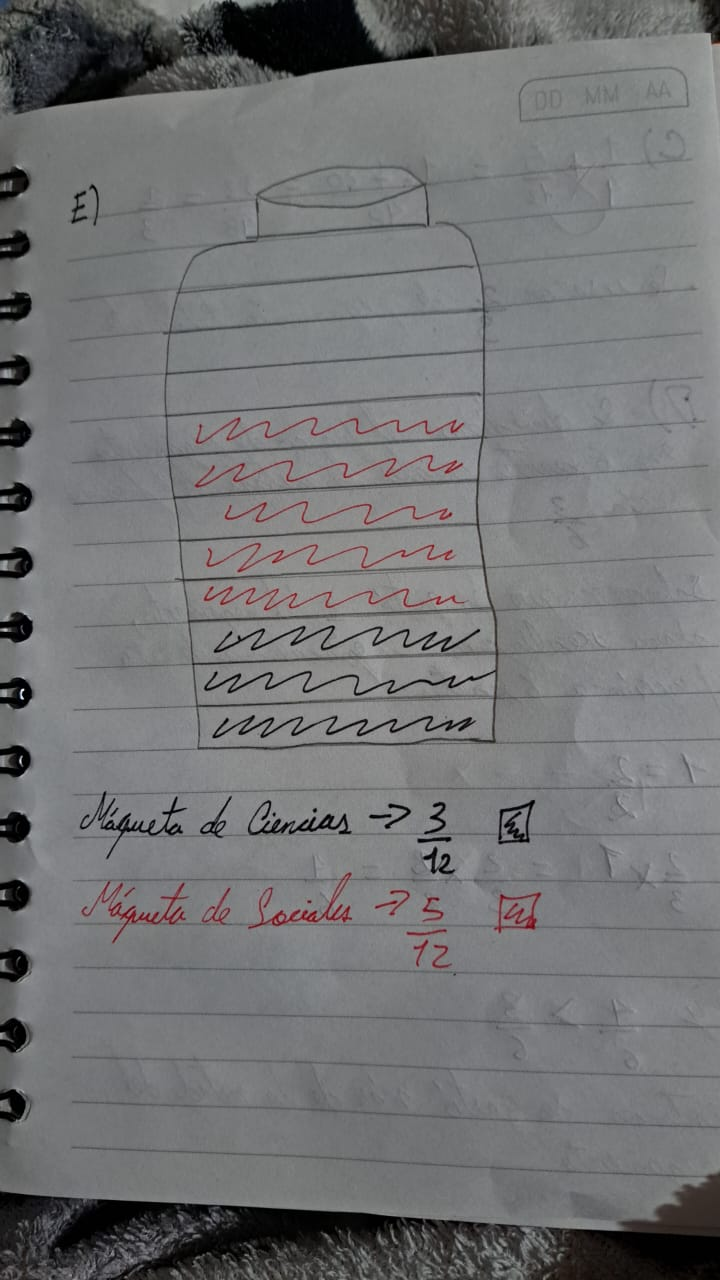
\includegraphics[scale=0.4]{lastpoint.jpg}


\end{document}